\chapter{Орбиты фотонов, пространство Риндлера и внутренняя область Шварцшильда}

Ньютоновская точечная масса и шварцшильдовская черная дыра опираются на одну и ту же идеализацию: вся гравитирующая масса сосредоточена в центре. Однако смысл этих центров очень различен. В ньютоновской механике частица даже с небольшим моментом импульса проходит мимо центра. В черной дыре, как только частица пересекла горизонт, сингулярность миновать невозможно. Понимание этого различия проведет нас через круговые орбиты, фотонную сферу и, наконец, к новому набору координат вблизи горизонта.

\section{Центр, который нельзя миновать}

Реальное ньютоновское вещество никогда не становится математической точкой. Давление, прочность материала и другие силы сопротивляются сжатию. Даже если мы все же используем точечную массу как идеализацию, падающая частица редко в нее попадает. Точно радиальная траектория может достичь \(r=0\), но малейшая поперечная скорость сообщает момент импульса. Тогда центробежный барьер уводит частицу в обход центра.

Общая теория относительности меняет вывод. Достаточно компактное тело может образовать черную дыру, и во внутренней области черной дыры ньютоновская возможность избежать центра, обойдя его, перестает работать. Причина глубже, чем просто более сильная сила: внутри горизонта уменьшение \(r\) соответствует направлению в будущее. Мы придем к этому утверждению постепенно, а не будем просто исходить из него.

\begin{classroomqa} \audiencequestion{Является ли ньютоновская трудность попадания в центр всего лишь следствием того, что оба объекта рассматриваются как точки?} \lecturerresponse{Точечная идеализация — часть сравнения, но она не исчерпывает всего различия. В ньютоновской механике любой ненулевой момент импульса позволяет орбите пройти вокруг точки. В релятивистской внутренней области сингулярность лежит в будущем любой падающей времениподобной траектории; угловое движение не может обеспечить уход. \lecturetimestamp{00:04:52--00:05:13}} \end{classroomqa}

\section{Горизонт и сингулярность}

Пока примем геометрию Шварцшильда как данную: \begin{equation}
d\tau^{2}
=
\left(1-\frac{2MG}{r}\right)dt^{2}
-
\frac{dr^{2}}{1-\frac{2MG}{r}}
-
r^{2}d\Omega^{2}.
\label{eq:l6-schwarzschild}
\end{equation} Уравнения поля, которые выделяют эту метрику, появятся позже. Наша ближайшая задача — понять, что говорит эта метрика.

Метрику на единичной сфере можно записать в виде \begin{equation}
d\Omega^{2}
=d\vartheta^{2}+\cos^{2}\vartheta\,d\phi^{2}
\label{eq:l6-angular-metric}
\end{equation} если \(\vartheta\) — широта, отсчитываемая от экваториальной плоскости. При более привычном полярном угле, отсчитываемом от оси, косинус заменяется синусом. Сферическая симметрия позволяет поместить любую орбиту в одну фиксированную плоскость, поэтому в вычислении ниже останется только одна угловая координата.

\begin{figure}[htbp] \centering
\includegraphics[width=0.88\textwidth]{lecture_06_figure_01.png} \caption{Метрика Шварцшильда и цилиндрическое пространственно-временное изображение поверхности \(r=2MG\). Центральная линия — это \(r=0\); красный цилиндр — горизонт в координатах Шварцшильда.} \lectureframe{00:09:45} \end{figure}

Вдали от источника \(2MG/r\) мало, и уравнение~\eqref{eq:l6-schwarzschild} приближается к метрике Минковского в сферических координатах. Выделяются два радиуса: \begin{equation}
r=2MG,
\qquad
r=0.
\end{equation} Их не следует путать. При \(r=2MG\) коэффициент при \(dt^{2}\) обращается в нуль, а коэффициент при \(dr^{2}\) расходится. Координатная система Шварцшильда становится сингулярной. Сама кривизна там остается конечной. Напротив, при \(r=0\) инварианты кривизны расходятся. Поле приливных сил растягивает протяженное тело в радиальном направлении и безгранично сжимает его в поперечном. Это физическая сингулярность, а не дефект координат.

\subsection{Два способа измерять время падения}

Для неподвижных часов вне горизонта \begin{equation}
d\tau
=
\sqrt{1-\frac{2MG}{r}}\,dt.
\label{eq:l6-static-clock}
\end{equation} При больших \(r\) имеет место \(d\tau\simeq dt\). Вблизи горизонта собственное время часов, удерживаемых при фиксированном \(r\), течет очень медленно по сравнению со шварцшильдовым временем, отсчитываемым далеко оттуда.

Те же координаты описывают радиальное падение так, что для достижения \(r=2MG\) требуется бесконечное значение \(t\). Собственное прошедшее время самого падающего конечно. Между этими утверждениями нет противоречия. Часы, которые несет падающий, измеряют собственное время вдоль его мировой линии. Это могут быть механические часы, световые часы из зеркал на концах метрового стержня, сердцебиение или последовательность физических процессов в мозге. Ничто из этого не измеряет удаленную координату \(t\). Различие между этими двумя часами станет видно на диаграмме вблизи горизонта.

\section{Круговое движение из действия по собственному времени}

Прежде чем вернуться к падению, решим другую задачу: при каких условиях массивная частица или фотон могут двигаться вокруг черной дыры по круговой орбите? Вычисление начинается с того же принципа действия, который используется для любой свободно движущейся релятивистской частицы, \begin{equation}
S=-m\int d\tau.
\label{eq:l6-particle-action}
\end{equation} Свет отклоняется Землей, но земное поле и близко не достаточно сильно, чтобы замкнуть световой луч в орбиту. Шварцшильдовский радиус Земли составляет всего лишь величину порядка сантиметра. Чтобы вопрос о сильном поле стал существенным, пришлось бы сжать всю Землю примерно до такого масштаба, то есть до размера небольшого ореха.

Положим \(c=1\), рассмотрим движение в экваториальной плоскости и определим \begin{equation}
F(r)=1-\frac{2MG}{r},
\qquad
G(r)=\frac{1}{F(r)}.
\label{eq:l6-fg}
\end{equation} Если взять в качестве параметра координатное время \(t\), то получим \begin{equation}
d\tau
=dt\sqrt{F-G\dot r^{\,2}-r^{2}\dot\theta^{\,2}},
\end{equation} и, следовательно, \begin{equation}
\mathcal L
=
-m\sqrt{F-G\dot r^{\,2}-r^{2}\dot\theta^{\,2}}.
\label{eq:l6-lagrangian}
\end{equation} Множитель \(m\) придает действию его обычную размерность — энергия, умноженная на время.

\begin{figure}[htbp] \centering
\includegraphics[width=0.76\textwidth]{lecture_06_figure_02.png} \caption{На доске шаг за шагом строится лагранжиан частицы с квадратным корнем. Полное выражение дано в уравнении~\eqref{eq:l6-lagrangian}.} \lectureframe{00:31:53} \end{figure}

Для любой обобщенной координаты \(q\), \begin{equation}
p_q=\frac{\partial\mathcal L}{\partial\dot q}.
\end{equation} Полезно сохранить обозначение \(\mathcal L\) для лагранжиана, а \(L\) — для момента импульса. При \begin{equation}
\Delta=F-G\dot r^{\,2}-r^{2}\dot\theta^{\,2},
\end{equation} два импульса равны \begin{align}
L=p_\theta
&=\frac{mr^{2}\dot\theta}{\sqrt{\Delta}},
\label{eq:l6-angular-momentum}\\
p_r
&=\frac{mG\dot r}{\sqrt{\Delta}}.
\label{eq:l6-radial-momentum}
\end{align} Радиальный импульс не сохраняется, потому что радиальная координата входит в лагранжиан. Угол \(\theta\) не входит, поэтому \(L\) сохраняется.

Явной зависимости от \(t\) в \(\mathcal L\) также нет. Поэтому гамильтониан сохраняется: \begin{align}
E=H
&=p_r\dot r+L\dot\theta-\mathcal L \\
&=\frac{mG\dot r^{\,2}}{\sqrt{\Delta}}
  +\frac{mr^{2}\dot\theta^{\,2}}{\sqrt{\Delta}}
  +m\sqrt{\Delta} \\
&=\frac{mF}{\sqrt{\Delta}}.
\label{eq:l6-energy-general}
\end{align} Это характерный ритм механики. Принцип задает действие; вычисление дает импульсы; затем симметрия превращает результат вычисления обратно в законы сохранения энергии и момента импульса. Можно было бы сразу решить все уравнения Эйлера--Лагранжа, но константы, даваемые вращательной симметрией и симметрией относительно сдвигов по времени, избавляют от значительной части этой работы.

\subsection{Энергия круговой орбиты}

Для круговой орбиты, \begin{equation}
\dot r=0.
\end{equation} Введем момент импульса на единицу массы, \begin{equation}
\lambda=\frac{L}{m}.
\end{equation} Уравнения~\eqref{eq:l6-angular-momentum} и \eqref{eq:l6-energy-general} принимают вид \begin{align}
\lambda
&=\frac{r^{2}\dot\theta}
{\sqrt{F-r^{2}\dot\theta^{\,2}}},
\label{eq:l6-lambda-circular}\\
E
&=\frac{mF}{\sqrt{F-r^{2}\dot\theta^{\,2}}}.
\label{eq:l6-energy-circular-first}
\end{align}

\begin{figure}[htbp] \centering
\includegraphics[width=0.82\textwidth]{lecture_06_figure_04.png} \caption{Удельный момент импульса и энергия для кругового движения в геометрии Шварцшильда. Сначала уравнение для момента импульса используется, чтобы исключить \(\dot\theta\) из выражения для энергии.} \lectureframe{00:39:14} \end{figure}

Возведя уравнение~\eqref{eq:l6-lambda-circular} в квадрат и решив его относительно угловой скорости, получаем \begin{equation}
\dot\theta^{\,2}
=
\frac{\lambda^{2}F}
{r^{2}\left(r^{2}+\lambda^{2}\right)}.
\label{eq:l6-angular-speed}
\end{equation} Подстановка в уравнение~\eqref{eq:l6-energy-circular-first} дает энергию, зависящую только от предполагаемого радиуса и фиксированного момента импульса: \begin{equation}
E(r,\lambda)
=m\sqrt{F(r)}\,\frac{\sqrt{r^{2}+\lambda^{2}}}{r}.
\label{eq:l6-circular-energy}
\end{equation}

Сделаем паузу для ньютоновского сравнения. В обычной круговой орбите угловая частота и тангенциальная скорость уменьшаются с ростом радиуса, но в момент импульса входит множитель радиуса. Поэтому о поведении \(L\) не следует судить только по угловой скорости. В релятивистской формуле эти множители остаются явными.

\section{Круговая орбита света}

Фотон имеет энергию и импульс, хотя его масса покоя равна нулю. Безмассовый предел уравнения~\eqref{eq:l6-circular-energy} поэтому нужно брать с осторожностью. Если \(m\) стремится к нулю при фиксированном \(\lambda\), то \(L=m\lambda\) тоже обращается в нуль. Вместо этого возьмем \begin{equation}
m\longrightarrow0,
\qquad
\lambda\longrightarrow\infty,
\qquad
L=m\lambda\ \text{fixed}.
\label{eq:l6-massless-limit}
\end{equation} Тогда доминирует член \(\lambda^{2}\), и энергия фотона принимает вид \begin{equation}
E_\gamma(r;L)
=L\,\frac{\sqrt{1-\frac{2MG}{r}}}{r}.
\label{eq:l6-photon-energy}
\end{equation} Множитель \(L\) умножает всю радиальную функцию. Он влияет на масштаб энергии, но не на радиус круговой орбиты.

\begin{figure}[htbp] \centering
\includegraphics[width=0.88\textwidth]{lecture_06_figure_05.png} \caption{Радиальный множитель в энергии фотона. Он обращается в нуль на горизонте, стремится к нулю при большом радиусе и имеет между ними один максимум.} \lectureframe{00:50:50} \end{figure}

При фиксированном \(L\) радиальное равновесие требует стационарной точки: \begin{equation}
\frac{d}{dr}
\left[
\frac{\sqrt{1-\frac{2MG}{r}}}{r}
\right]=0.
\end{equation} Дифференцируя, \begin{equation}
-\frac{\sqrt{1-\frac{2MG}{r}}}{r^{2}}
+
\frac{MG}
{r^{3}\sqrt{1-\frac{2MG}{r}}}
=0,
\end{equation} и, следовательно, \begin{equation}
r=3MG.
\label{eq:l6-photon-sphere}
\end{equation} Этот радиус в полтора раза больше радиуса Шварцшильда. Его обычно называют фотонной сферой.

Стационарная точка является максимумом, поэтому круговая фотонная орбита неустойчива. Фотон, помещенный точно на \(3MG\), остается там. Сколь угодно малое радиальное смещение в конце концов уводит его от максимума. Сразу снаружи фотонной сферы луч может пройти через очень большой угол, возможно много раз обогнув дыру, прежде чем уйти. Сразу внутри нее почти касательный луч может несколько раз обернуться, а затем упасть через горизонт.

\begin{figure}[htbp] \centering
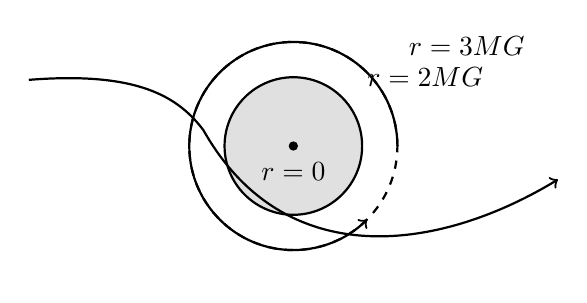
\begin{tikzpicture}[scale=1.12]
\fill[black!12] (0,0) circle (0.78);
\draw[thick] (0,0) circle (0.78);
\draw[dashed,thick] (0,0) circle (1.18);
\fill (0,0) circle (1.5pt);
\draw[->,thick] (1.18,0) arc (0:315:1.18);
\draw[->,thick] (-3.0,0.75)
  .. controls (-1.75,0.85) and (-1.30,0.55) .. (-1.02,0.18)
  .. controls (-0.10,-1.45) and (1.65,-1.20) .. (3.0,-0.38);
\node[right] at (0.73,0.78) {\(r=2MG\)};
\node[right] at (1.20,1.13) {\(r=3MG\)};
\node[below] at (0,-0.08) {\(r=0\)};
\end{tikzpicture} \caption{Горизонт, фотонная сфера и сильно отклоненный луч. Лучи, сколь угодно близкие к неустойчивой круговой орбите, могут накапливать сколь угодно большое отклонение, прежде чем уйти или упасть внутрь.} \end{figure}

\begin{classroomqa}
\audiencequestion{Почему мы фиксируем угловой момент и как он связан с частотой фотона и траекторией его подлета?}
\lecturerresponse{Каждый луч несет сохраняющийся угловой момент относительно черной дыры. Его частота фиксирует модуль его линейного импульса, а смещение относительно центра помогает определить \(L\). Вне круговой орбиты радиус и угловой момент можно выбирать независимо. Требование круговой фотонной орбиты связывает движение с единственным радиусом \(3MG\), а разложение на множители в уравнении~\eqref{eq:l6-photon-energy} показывает, что этот радиус не зависит от величины \(L\).
\lecturetimestamp{00:54:43--00:57:02}}
\end{classroomqa}

\begin{classroomqa}
\audiencequestion{Почему максимум энергии определяет орбиту?}
\lecturerresponse{После исключения углового движения при фиксированном \(L\) оставшаяся функция играет роль эффективной радиальной энергии. Стационарная точка задает радиальное равновесие. Минимум был бы устойчивым; эта точка является максимумом и потому соответствует неустойчивой круговой орбите. Нет никакого противоречия в том, чтобы одновременно называть ее равновесной и неустойчивой.
\lecturetimestamp{00:57:51--00:58:54}}
\end{classroomqa}

Массивная частица может иметь времениподобные круговые орбиты вне \(3MG\), хотя ближайшие к фотонной сфере из них неустойчивы. Безмассовая частица имеет только круговую орбиту при \(3MG\). Внутри фотонной сферы фотон, движущийся по касательной, падает внутрь; у объекта, движущегося медленнее, шансов удержаться на такой орбите не больше. Это утверждение относится к угловому движению. Вне горизонта луч, направленный достаточно сильно наружу, все еще может уйти, даже если его начальный радиус меньше \(3MG\).

\section{Что делает черная дыра с изображением}

Фотонная сфера объясняет, почему черная дыра — не просто темный диск, наложенный на в остальном неизменное небо. Свет от фонового объекта может дойти до наблюдателя по нескольким путям. Один луч может пройти с одной стороны дыры, другой — с другой, а еще другие могут обойти дыру один или несколько раз. В результате возможны смещенные изображения, дублированные изображения, кольца и бесконечная последовательность все более тонких и все более тусклых изображений, связанных с дополнительными обходами. Точная картина сложна, но ее происхождение уже заключено в неустойчивой орбите.

Когда источник, линза и наблюдатель достаточно хорошо выстроены вдоль одной прямой, изображение может образовать кольцо Эйнштейна. Кольца гравитационного линзирования наблюдаются в природе. Полное изображение черной дыры требует интегрирования нулевых геодезических для многих начальных направлений; это вычисление хорошо подходит для компьютера.

\begin{classroomqa}
\audiencequestion{Относится ли эта оптическая граница к фотонной сфере или к горизонту?}
\lecturerresponse{Они играют разные роли. Горизонт при \(2MG\) — это причинная граница: изнутри него не выходит ни один направленный в будущее сигнал. Фотонная сфера при \(3MG\) управляет касательным движением и сильным линзированием. Между этими двумя радиусами направленный радиально наружу луч может уйти, тогда как касательный луч падает внутрь. При промежуточных направлениях луч может сделать петлю, прежде чем уйти или быть захваченным.
\lecturetimestamp{01:02:47--01:03:40}}
\end{classroomqa}

\begin{classroomqa}
\audiencequestion{Можно ли вычислить общую световую траекторию, а не просто набросать ее?}
\lecturerresponse{Да. Подставьте нулевое условие в уравнения геодезических или Эйлера--Лагранжа и проинтегрируйте их с выбранными начальными данными. Эти уравнения концептуально не новы, но трассировка лучей алгебраически громоздка, поэтому для получения изображения практическим методом является численный расчет.
\lecturetimestamp{01:03:48--01:04:27}}
\end{classroomqa}

\begin{classroomqa}
\audiencequestion{Сделало бы прямое применение уравнений Эйлера--Лагранжа вычисление круговой орбиты более сложным?}
\lecturerresponse{Оно дало бы тот же результат. Действие является правильной исходной точкой в обоих методах, но циклические координаты выявляют сохраняющиеся энергию и угловой момент. Использовать сначала эти константы — более короткий путь к условию круговой орбиты.
\lecturetimestamp{01:04:33--01:05:49}}
\end{classroomqa}

\section{Метрика вблизи горизонта — пространство Риндлера}

Теперь вернемся к горизонту. Коэффициенты метрики Шварцшильда там, по-видимому, расходятся или обращаются в нуль, а при пересечении горизонта их знаки меняются местами. И все же падающий наблюдатель не встречает на этой поверхности никакой расходящейся локальной кривизны. Принцип эквивалентности объясняет, как оба эти утверждения могут быть верны.

Начнем с двумерного пространства-времени Минковского:
\begin{equation}
d\tau^{2}=dT^{2}-dX^{2}.
\end{equation}
В правом клине Риндлера зададим
\begin{equation}
X=\rho\cosh\omega,
\qquad
T=\rho\sinh\omega.
\label{eq:l6-rindler-map}
\end{equation}
Кривые с постоянным \(\rho\) удовлетворяют соотношению
\begin{equation}
X^{2}-T^{2}=\rho^{2},
\end{equation}
поэтому это гиперболы, мировые линии равномерно ускоренных наблюдателей.
Подставляя уравнение~\eqref{eq:l6-rindler-map} в плоскую метрику, получаем
\begin{equation}
d\tau^{2}
=\rho^{2}d\omega^{2}-d\rho^{2}.
\label{eq:l6-rindler-metric}
\end{equation}
Теперь положим
\begin{equation}
\rho^{2}=4\xi,
\qquad
\omega=\frac{t}{2}.
\label{eq:l6-rindler-rescale}
\end{equation}
Поскольку \(d\rho^{2}=d\xi^{2}/\xi\), уравнение~\eqref{eq:l6-rindler-metric}
принимает вид
\begin{equation}
d\tau^{2}
=\xi\,dt^{2}-\frac{d\xi^{2}}{\xi}.
\label{eq:l6-xi-metric}
\end{equation}

\begin{classroomqa}
\audiencequestion{Куда делись угловые, или поперечные, координаты?}
\lecturerresponse{Их лишь опустили. Мы рассматриваем локальную плоскость \(t\)-\(r\), в которой проявляется поведение при пересечении горизонта. Два поперечных направления остаются регулярными и могут быть возвращены; они не меняют анализируемую координатную сингулярность.
\lecturetimestamp{01:16:27--01:16:47}}
\end{classroomqa}

Чтобы сравнить со Шварцшильдом, выберем единицы, в которых \(2MG=1\). Радиальная часть уравнения~\eqref{eq:l6-schwarzschild} имеет вид
\begin{equation}
d\tau^{2}
=
\frac{r-1}{r}\,dt^{2}
-
\frac{r}{r-1}\,dr^{2}.
\end{equation}
Совсем близко к \(r=1\) малый числитель \(r-1\) необходимо сохранить, тогда как множители \(r\), которые в остальном безвредны, можно заменить единицей. Поэтому
\begin{equation}
d\tau^{2}
\simeq
(r-1)\,dt^{2}
-
\frac{dr^{2}}{r-1}.
\end{equation}
При
\begin{equation}
\xi=r-1,
\end{equation}
это в точности уравнение~\eqref{eq:l6-xi-metric}. Геометрия Шварцшильда вблизи горизонта локально является риндлеровским описанием плоского пространства-времени.

\begin{classroomqa}
\audiencequestion{Как это могут быть ускоренные координаты, если само пространство-время плоское?}
\lecturerresponse{Ускорение относится к наблюдателю, а не обязательно к кривизне. Мировая линия при фиксированном \(\rho\) равномерно ускорена в пространстве-времени Минковского. Точно так же наблюдатель на фиксированном радиусе вблизи черной дыры должен удерживаться от свободного падения. Принцип эквивалентности делает локальные описания совпадающими, хотя полное пространство-время Шварцшильда искривлено.
\lecturetimestamp{01:22:19--01:24:06}}
\end{classroomqa}

\section{Пересечение горизонта Риндлера}

Формулы для правого клина охватывают только область \(\xi>0\):
\begin{equation}
X=2\sqrt{\xi}\cosh\frac{t}{2},
\qquad
T=2\sqrt{\xi}\sinh\frac{t}{2}.
\label{eq:l6-rindler-outside}
\end{equation}
Поверхность \(\xi=0\) — это нулевая прямая \(X=T\). Чтобы продолжить в будущий клин, положим
\begin{equation}
\zeta=-\xi>0
\end{equation}
и поменяем местами роли гиперболических функций:
\begin{equation}
T=2\sqrt{\zeta}\cosh\frac{t}{2},
\qquad
X=2\sqrt{\zeta}\sinh\frac{t}{2}.
\label{eq:l6-rindler-inside}
\end{equation}
Метрика по-прежнему имеет вид
\begin{equation}
d\tau^{2}
=\xi\,dt^{2}-\frac{d\xi^{2}}{\xi},
\end{equation}
но при \(\xi<0\) коэффициент при \(dt^{2}\) отрицателен, а коэффициент при \(d\xi^{2}\) положителен. Координата \(\xi\), а значит и радиальное направление Шварцшильда, стала времениподобной; \(t\) стала пространственноподобной.

\begin{figure}[htbp]
\centering
\includegraphics[width=0.88\textwidth]{lecture_06_figure_06.png}
\caption{Клины Риндлера, их нулевые границы и продолжение от
\(\xi>0\) к \(\xi<0\). На доске также записаны
\(\rho^{2}=4\xi\) и \(\omega=t/2\).}
\lectureframe{01:29:40}
\end{figure}

\begin{classroomqa}
\audiencequestion{Движутся ли некоторые кривые на этой координатной диаграмме быстрее света?}
\lecturerresponse{Линия координатной сетки не обязана быть мировой линией материального объекта. Ее наклон в координатах может выглядеть сверхсветовым, не нарушая причинности. Физические световые лучи по-прежнему идут по нулевым линиям, а физические частицы остаются внутри своих локальных световых конусов.
\lecturetimestamp{01:28:44--01:29:08}}
\end{classroomqa}

Продолжая двигаться дальше во внутреннюю область Шварцшильда, мы в конце концов приходим к \(r=0\). Эта граница пространственноподобна. Поэтому ее лучше описывать как время, а не как место: каждая направленная в будущее времениподобная или нулевая траектория внутри черной дыры достигает ее. Место можно обойти. Свое будущее обойти нельзя.

\begin{classroomqa}
\audiencequestion{Можно ли просто продолжить диаграмму через \(r=0\) к отрицательным \(r\), и остается ли \(r=0\) центром?}
\lecturerresponse{Координатная диаграмма может наводить на мысль просто продолжить линию, но классическое решение Шварцшильда оканчивается на сингулярности кривизны. \(r=0\) все еще можно называть центром, но это очень необычный центр: во внутренней области он является пространственноподобной будущей границей. Регулярного прохода через него в область отрицательного радиуса нет.
\lecturetimestamp{01:32:16--01:34:06}}
\end{classroomqa}

\begin{classroomqa}
\audiencequestion{Являются ли диагональные оси на диаграмме Риндлера светоподобными, и может ли падающий наблюдатель пересечь горизонт при конечном значении ускоренного времени?}
\lecturerresponse{Да, границы клина — нулевые линии. Мировая линия свободно падающего наблюдателя пересекает такую линию в обычном конечном событии и за конечное собственное время. Ускоренная координата \(t\), или эквивалентно \(\omega\), неограниченно возрастает вдоль внешнего описания при постоянном \(\rho\); бесконечной становится именно эта координатная параметризация, а не событие пересечения.
\lecturetimestamp{01:34:26--01:35:03}}
\end{classroomqa}

\section{Алиса снаружи, а Боб падает}

Пусть Алиса остается снаружи на фиксированном радиусе, удерживаемая от свободного падения, а Боб свободно падает. Вблизи горизонта Алиса движется по риндлероподобной гиперболе. Ее срезы при постоянном \(t\) сгущаются все ближе и ближе к нулевой границе. Каждое событие на мировой линии Боба, которому Алиса приписывает конечное \(t\), лежит вне горизонта, поэтому его пересечению она никогда не приписывает конечное шварцшильдовское время.

У Боба есть часы, измеряющие собственное время. Его траектория пересекает светоподобную линию за конечный интервал, отсчитанный этими часами. При пересечении не возникает никаких локально расходящихся величин. Горизонт имеет решающее глобальное значение, но локально он ничем не примечателен.

\begin{figure}[htbp]
\centering
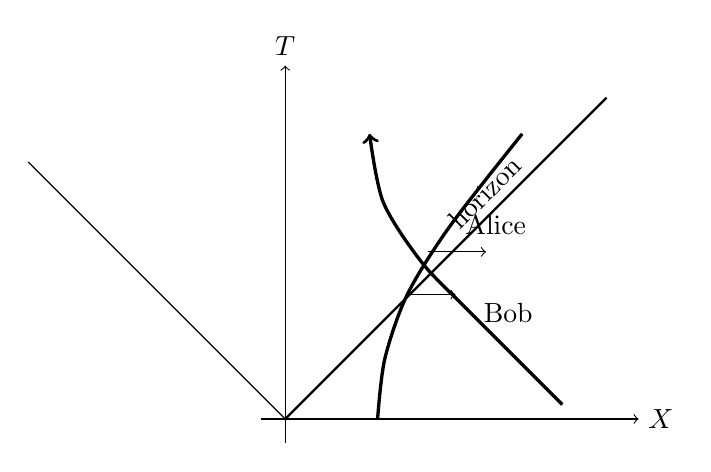
\begin{tikzpicture}[scale=1.02]
\draw[->] (-0.3,0) -- (4.4,0) node[right] {\(X\)};
\draw[->] (0,-0.3) -- (0,4.4) node[above] {\(T\)};
\draw[thick] (0,0) -- (4.0,4.0);
\draw[thin] (0,0) -- (-3.2,3.2);
\node[rotate=45,above] at (2.65,2.65) {horizon};
\draw[very thick]
  plot[smooth] coordinates {(1.15,0.0) (1.24,0.75) (1.52,1.55)
  (2.05,2.40) (2.95,3.55)};
\node[right] at (2.12,2.42) {Alice};
\draw[very thick,->]
  plot[smooth] coordinates {(3.45,0.18) (2.85,0.78) (2.25,1.38)
  (1.70,1.95) (1.22,2.70) (1.05,3.55)};
\node[right] at (2.35,1.32) {Bob};
\draw[->] (1.52,1.55) -- (2.12,1.55);
\draw[->] (1.78,2.08) -- (2.50,2.08);
\end{tikzpicture}
\caption{Ускоренная мировая линия Алисы во внешней области и свободно падающая мировая линия Боба. Координатные срезы Алисы приближаются к горизонту; Боб пересекает его за конечное собственное время.}
\end{figure}

\begin{classroomqa}
\audiencequestion{Что видит Боб, когда оглядывается на Алису, и что происходит с его часами после пересечения?}
\lecturerresponse{Боб видит, как Алиса удаляется, сохраняя ускорение, необходимое, чтобы удерживать её снаружи, но при пересечении он не наблюдает никакого сингулярного события. Алису можно удерживать на фиксированном радиусе; орбита — другая возможная постановка. Его часы продолжают нормально отсчитывать собственное время \(\tau\). Внутри утверждение о том, что радиальная координата является времениподобной, описывает причинную геометрию; это не означает буквально, что его наручные часы превращаются в метровую линейку. Его мировая линия в конце концов оканчивается в \(r=0\).
\lecturetimestamp{01:39:51--01:44:45}}
\end{classroomqa}

Светоподобная линия теперь распознаётся как сам горизонт, а не просто как одна точка, где один из координатных коэффициентов ведёт себя аномально. Вне него одно семейство радиальных световых лучей идёт наружу. Внутри него оба направления будущего светового конуса ведут к меньшим \(r\). Всякая направленная в будущее траектория массивной частицы должна оставаться между этими светоподобными направлениями и потому достигает сингулярности.

\section{Сигналы, красное смещение и формирующийся горизонт}

Предположим, что коллапсирующее вещество испускает регулярную последовательность световых импульсов. Далёкий наблюдатель принимает более поздние импульсы через всё большие интервалы. Их частоты смещаются от оптического диапазона к инфракрасному, микроволновому, радиодиапазону и к ещё большим длинам волн. В идеализированном классическом расчёте внешний наблюдатель может и дальше соотносить всё более поздние сигналы с веществом, приближающимся к горизонту, но на практике источник быстро становится слишком красносмещённым и слишком тусклым, чтобы его можно было обнаружить.

\begin{classroomqa}
\audiencequestion{Во время коллапса видит ли внешний наблюдатель, как всё вещество просто застывает на горизонте?}
\lecturerresponse{В шварцшильдовом времени поверхность коллапсирующего вещества асимптотически приближается к горизонту и кажется всё более застывающей. То, что действительно наблюдается, кодируется световыми сигналами, и эти сигналы становятся всё более запаздывающими, красносмещёнными и слабыми. Это координатное описание не говорит, что для падающего вещества проходит бесконечное собственное время.
\lecturetimestamp{01:47:06--01:48:11}}
\end{classroomqa}

\begin{classroomqa}
\audiencequestion{Может ли достаточно поздний наблюдатель восстановить всю историю падения?}
\lecturerresponse{Только по сигналам, которые были испущены и сумели достичь наблюдателя. Последовательные импульсы разделены всё большими интервалами и всё сильнее красносмещены. Идеальный наблюдатель с неограниченной чувствительностью мог бы прослеживать классический сигнал до всё больших длин волн; практический наблюдатель видит, как объект постепенно исчезает из виду.
\lecturetimestamp{01:48:13--01:52:00}}
\end{classroomqa}

\begin{classroomqa}
\audiencequestion{Что именно имеется в виду, когда говорят, что сингулярность — это время, а не место?}
\lecturerresponse{Поверхность \(r=0\) пространственноподобна. Оказавшись внутри горизонта, любая направленная в будущее времениподобная или нулевая кривая оканчивается на ней. Пространственного положения можно избежать, выбрав другой путь; будущей границы нельзя избежать, продолжая следовать вдоль мировой линии, направленной в будущее.
\lecturetimestamp{01:52:02--01:53:10}}
\end{classroomqa}

Как же тогда может образоваться чёрная дыра или увеличиться её масса, если внешний наблюдатель никогда не видит, как вещество пересекает горизонт? Рассмотрим коллапсирующую сферическую оболочку. Глобальный горизонт не ждёт в виде заранее существующей материальной поверхности на одном фиксированном радиусе. Он начинается в центре и растёт наружу, встречаясь с коллапсирующей оболочкой по мере формирования области чёрной дыры. Во внешнем шварцшильдовом описании оболочка всё так же асимптотически приближается к конечному горизонту. Полная картина пространства-времени, включая то, как горизонт определяется глобально, составляет предмет следующей лекции.

\begin{figure}[htbp]
\centering
\includegraphics[width=0.90\textwidth]{lecture_06_figure_07.png}
\caption{Коллапсирующая оболочка и горизонт, растущий наружу из центра ей навстречу. Этот рисунок — предварительный набросок глобальной геометрии коллапса, которая будет развита в следующей лекции.}
\lectureframe{01:57:25}
\end{figure}

\begin{classroomqa}
\audiencequestion{Если во внешнем координатном времени ничто не пересекает горизонт, как чёрная дыра может образоваться или расти?}
\lecturerresponse{Посылка смешивает координатное утверждение с глобальным. Коллапсирующее вещество достигает соответствующей области за конечное собственное время, тогда как горизонт событий определяется причинной структурой всего пространства-времени. В модели оболочки он начинается в центре и растёт наружу навстречу оболочке. Запаздывающий и красносмещённый вид, открывающийся внешнему наблюдателю, всё же согласуется с этим глобальным горизонтом.
\lecturetimestamp{01:53:11--01:57:34}}
\end{classroomqa}

\section{Направления выхода между двумя сферами}

Горизонт и фотонная сфера разбивают задачу о лучах на различные случаи. Для радиусов
\begin{equation}
2MG<r<3MG,
\end{equation}
световой луч, выходящий радиально наружу, может уйти на бесконечность. Тангенциальный луч не может; он падает внутрь. Между этими направлениями имеется конус выхода. Ближе к горизонту он сужается вокруг радиального направления наружу. После пересечения горизонта он полностью замыкается.

\begin{classroomqa}
\audiencequestion{Может ли источник света между горизонтом и фотонной сферой послать какой-либо сигнал наружу?}
\lecturerresponse{Да. Достаточно радиально направленный наружу световой луч уйдёт, пока событие его испускания находится вне \(2MG\). Утверждение о том, что угловое движение внутри \(3MG\) ведёт внутрь, не запрещает радиальный уход. Исход зависит от направления испускания, и конус допустимых наружных направлений сужается по мере приближения источника к горизонту.
\lecturetimestamp{01:57:34--01:59:48}}
\end{classroomqa}

\begin{classroomqa}
\audiencequestion{Может ли луч, приходящий снаружи, пройти внутрь фотонной сферы, развернуться и снова выйти?}
\lecturerresponse{Не по нулевой геодезической обсуждаемого типа. В точке разворота радиальная скорость была бы равна нулю, так что луч на мгновение стал бы тангенциальным на радиусе меньше \(3MG\); там угловая траектория падает внутрь, а не возвращается наружу. Тем не менее источник, уже находящийся между двумя сферами, может до пересечения горизонта испустить достаточно радиальный луч наружу.
\lecturetimestamp{01:59:49--02:01:27}}
\end{classroomqa}

Последний вопрос намеренно проработан менее полно. Представьте, что Алису и Боба обоих удерживают на одном и том же радиусе вне горизонта. Находящиеся близко друг к другу наблюдатели, разумеется, могут обмениваться сигналами. Если они далеко разнесены по сфере, прямой светоподобный путь и его предельный угловой диапазон требуют явного геодезического расчёта. На занятии предлагают косвенный маршрут: послать сообщение почти радиально наружу к ретранслятору на более безопасном радиусе, передать его там вокруг сферы и послать обратно внутрь. В другом варианте брошенный наружу объект или сигнал разворачивается и возвращается. Эти маршруты показывают, почему невозможность тангенциальной круговой орбиты сама по себе не запрещает всякую связь между внешними наблюдателями.

\begin{classroomqa}
\audiencequestion{Могут ли два наблюдателя, удерживаемые на одном и том же близком к горизонту радиусе, обмениваться сигналами вокруг чёрной дыры?}
\lecturerresponse{Локально — да. Для далеко разнесённых или диаметрально противоположных наблюдателей предельный угловой разнос, допускающий прямой путь, на лекции не был вычислен и не должен возводиться в ранг теоремы. Сначала обсуждение оставляет этот вопрос об угловой геодезической открытым, а затем замечает, что косвенный сигнал может уйти почти радиально наружу, быть ретранслирован на большем радиусе по кругу и вернуться. По мере приближения к горизонту угловой диапазон, полезный для прямой связи, становится всё уже, но вне горизонта путь наружу остаётся доступным.
\lecturetimestamp{02:01:29--02:04:17}}
\end{classroomqa}

Следующий шаг — заменить эти пригоризонтные наброски глобальной геометрией коллапсирующего тела и точно увидеть, как растёт горизонт событий.